\section{Introducción}
El presente trabajo tiene como objetivo implementar en una fpga un modo gráfico llamado \textbf{Mode 7}. Este modo gráfico tiene sus orígenes en la consola \textbf{SNES} (Super Nintendo Entertainment System), cuya aparición fue en el año 1990. Este modo gráfico permite realizar transformaciones de rotación (sobre un punto-origen), traslación y escalado a una imagen, logrando distintos efectos. Para ello se valía de un circuito en hardware especializado, que permitía lograr los cálculos en la velocidad en tiempo real para renderizar imágenes de una manera que no se había conseguido hasta el momento en consolas hogareñas. Algunos videojuegos que implementan Mode 7 son Super Castlevania 4 y Super Mario World.

\begin{center}
{
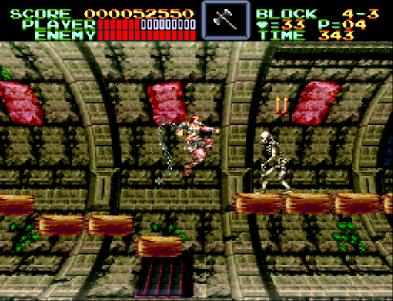
\includegraphics[scale=0.5]{castlevania.jpg}
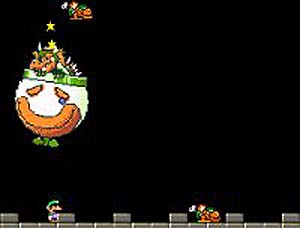
\includegraphics[scale=0.5]{mario.jpg}
}
\end{center}   
